\documentclass[aspectratio=169,11pt]{beamer}
% ==========================================================================
%  KSA lecture-slide theme  =  stock beamer "Boadilla"  +  KSA colour theme
%  brand colours sampled from the official KSA symbol mark:
%    Deep Prussian Blue  #2E3192   (지성 - intellect)
%    Golden Gray         #D6CBB1   (감성 - sensibility)
%  Engine: XeLaTeX.  Usage:
%    \documentclass[aspectratio=169,11pt]{beamer}
%    \input{../../theme/ksa-theme.tex}
%  Each deck lives in its own slides/kor/<deck>/ folder together with its
%  own images; ../../figs/ is kept only as a fallback for the shared cache.
% ==========================================================================

\usepackage{fontspec}
\usepackage{amsmath,amssymb}
\usepackage{graphicx}
\graphicspath{{figs/}{./}{../../../figs/}}
\usepackage{booktabs}
\usepackage{listings}
\usepackage{varwidth}

% ---- fonts (no ctex/xeCJK on this box -> fontspec drives CJK directly) -----
\defaultfontfeatures{Ligatures=TeX}
\setmainfont{Noto Sans CJK KR}
\setsansfont{Noto Sans CJK KR}
\setmonofont{Noto Sans Mono CJK KR}[Scale=0.92]

% ---- base theme: stock Boadilla ------------------------------------------
\usetheme{Boadilla}
\usefonttheme{professionalfonts}
\setbeamertemplate{navigation symbols}{}

% ---- KSA colour theme (recolour the stock theme) --------------------------
\definecolor{ksablue}{HTML}{2E3192}
\definecolor{ksabluedk}{HTML}{20226A}
\definecolor{ksagold}{HTML}{D6CBB1}
\definecolor{ksagolddk}{HTML}{A9976B}
\definecolor{ksared}{HTML}{C0392B}
\definecolor{ksagray}{HTML}{5B5B5B}

\setbeamercolor{structure}{fg=ksablue}
\setbeamercolor{alerted text}{fg=ksared}

\setbeamercolor{palette primary}{fg=white,           bg=ksablue}
\setbeamercolor{palette secondary}{fg=white,         bg=ksablue!85!black}
\setbeamercolor{palette tertiary}{fg=white,          bg=ksabluedk}
\setbeamercolor{titlelike}{fg=ksablue}
\setbeamercolor{frametitle}{fg=ksablue,bg=}
\setbeamercolor{title}{fg=ksablue}
\setbeamercolor{author}{fg=ksagray}
\setbeamercolor{institute}{fg=ksagray}
\setbeamercolor{block title}{fg=white,bg=ksablue}
\setbeamercolor{block body}{fg=black!85,bg=ksablue!6}
\setbeamercolor{item}{fg=ksablue}
\setbeamercolor{section in toc}{fg=black!85}

\setbeamerfont{frametitle}{series=\bfseries}
\setbeamerfont{title}{series=\bfseries}

% ---- footline:  KSA mark | "Made by ..." | n / N   (matches reference) ----
\newcommand{\ksacredit}{}
\setbeamertemplate{footline}{%
  \hbox{%
    \begin{beamercolorbox}[wd=.18\paperwidth,ht=2.6ex,dp=1.5ex,leftskip=1.1em]{}%
      \raisebox{-0.35ex}{\includegraphics[height=2.0ex]{ksa-logo.png}}%
    \end{beamercolorbox}%
    \begin{beamercolorbox}[wd=.64\paperwidth,ht=2.6ex,dp=1.5ex,center]{}%
      {\scriptsize\color{ksagray}\ksacredit}%
    \end{beamercolorbox}%
    \begin{beamercolorbox}[wd=.18\paperwidth,ht=2.6ex,dp=1.5ex,rightskip=1.1em]{}%
      \hfill{\scriptsize\color{ksablue}\insertframenumber\,/\,\inserttotalframenumber}%
    \end{beamercolorbox}%
  }%
  \vskip2pt
}

% ---- section divider: stock \sectionpage, KSA-coloured -------------------
\setbeamertemplate{section page}{%
  \begingroup\centering
    {\color{ksagolddk}\rule{0.16\paperwidth}{1pt}}\par\vskip1.0em
    {\usebeamerfont{title}\color{ksablue}\insertsectionhead\par}\vskip1.0em
    {\color{ksagolddk}\rule{0.16\paperwidth}{1pt}}\par
  \endgroup
}
\AtBeginSection[]{\begin{frame}[plain,noframenumbering]\vfill\sectionpage\vfill\end{frame}}

% ---- code listings ------------------------------------------------------------
\lstdefinestyle{ksa}{%
  basicstyle=\ttfamily\scriptsize,
  keywordstyle=\color{ksablue}\bfseries,
  commentstyle=\color{ksagray}\itshape,
  stringstyle=\color{ksagolddk},
  numberstyle=\tiny\color{ksagray},
  backgroundcolor=\color{ksablue!6},
  frame=leftline, framerule=1.4pt, rulecolor=\color{ksablue},
  xleftmargin=1em, aboveskip=0.8em, belowskip=0.4em,
  showstringspaces=false, breaklines=true, language=Python,
}
\lstset{style=ksa}

% ---- handy macros -----------------------------------------------------------
\newcommand{\kb}[1]{\textbf{\color{ksablue}#1}}   % blue keyword
\newcommand{\kq}[1]{\textbf{\color{ksared}#1}}    % red key-question

\setbeamerfont{title}{series=\bfseries,size=\fontsize{24}{30}\selectfont}
\setbeamerfont{subtitle}{series=\bfseries,size=\fontsize{14}{18}\selectfont}
\setbeamerfont{author}{size=\normalsize}
\setbeamerfont{institute}{size=\small}
\graphicspath{{figs/}{../../../../assets/}}
% 한글 글꼴에 이탤릭이 없어서 기울임은 FakeSlant 로 만든다 (\slant{...})
\newfontfamily\slantfont{Noto Sans CJK KR}[FakeSlant=0.18, BoldFeatures={FakeSlant=0.18}]
\newcommand{\slant}[1]{{\slantfont #1}}
\makeatletter
\newcommand{\markpage}[1]{\protected@write\@auxout{}{\string\newlabel{#1}{{\the\c@framenumber}{}}}\hypertarget{#1}{}}
\newcommand{\pref}[1]{\hyperlink{#1}{\textcolor{ksagolddk}{(p.\ref{#1})}}}
\makeatother

\renewcommand{\ksacredit}{Machine Learning 1 \,\textperiodcentered\, 이 수업은 무엇을 하는가}
\title{머신러닝 1: 이 수업은 무엇을 하는가}
\subtitle{AI는 과학의 산물일까, 공학의 산물일까?}
\author{Machine Learning 1}
\institute{한국과학영재학교 (KSA)}
\date{}
\begin{document}
\begin{frame}[plain,noframenumbering]\titlepage\end{frame}

% --- 오늘의 질문
\begin{frame}{오늘의 질문}
\markpage{question}
\vfill
\centering{\LARGE\kq{AI는 과학의 산물일까, 공학의 산물일까?}}\par\vskip1.4em
{\Large\slant{``\textbf{만들 수 없는 것}은 \textbf{이해하지 못한 것}이다.''}}\par\vskip0.3em
{\normalsize\slant{What I cannot create, I do not understand.}}\par\vskip0.6em
{\small --- 리처드 파인먼 (1965 노벨 물리학상), 1988년 세상을 떠날 때 칠판에 남아 있던 문장}\par\vskip1.0em
{\large\color{gray} 그런데 우리는 AI를 \textbf{만들 줄 안다}. 그러면 AI를 \textbf{이해한} 걸까?}
\vfill
\note{첫 시간이니 어려운 공식 대신 질문 하나로 시작하겠습니다. AI는 과학의 산물일까요, 공학의 산물일까요? 노벨 물리학상을 받은 리처드 파인먼이 세상을 떠날 때 칠판에는 이 문장이 남아 있었습니다. 만들 수 없는 것은 이해하지 못한 것이다. 이해했다면 처음부터 직접 만들어 낼 수 있어야 한다는 뜻입니다. 그런데 우리는 AI를 만들 줄 압니다. 그러면 AI를 이해한 걸까요? 아닙니다. 만들 수 있다고 해서 이해한 것은 아닙니다. 우리는 LLM을 만들 줄 알지만, 그 안에서 무슨 일이 일어나는지, 왜 이렇게 잘 되는지는 아직 잘 모릅니다. 만드는 것은 공학이고 이해하는 것은 과학이라면, 지금의 AI는 그 사이 어딘가에 있습니다. 오늘 짧은 역사를 같이 보면서 이 질문에 각자 답을 정해 보세요. 수업 끝에 다시 묻겠습니다.}
\end{frame}

% --- 우스갯소리
\begin{frame}{우스갯소리로는}
\vfill
\centering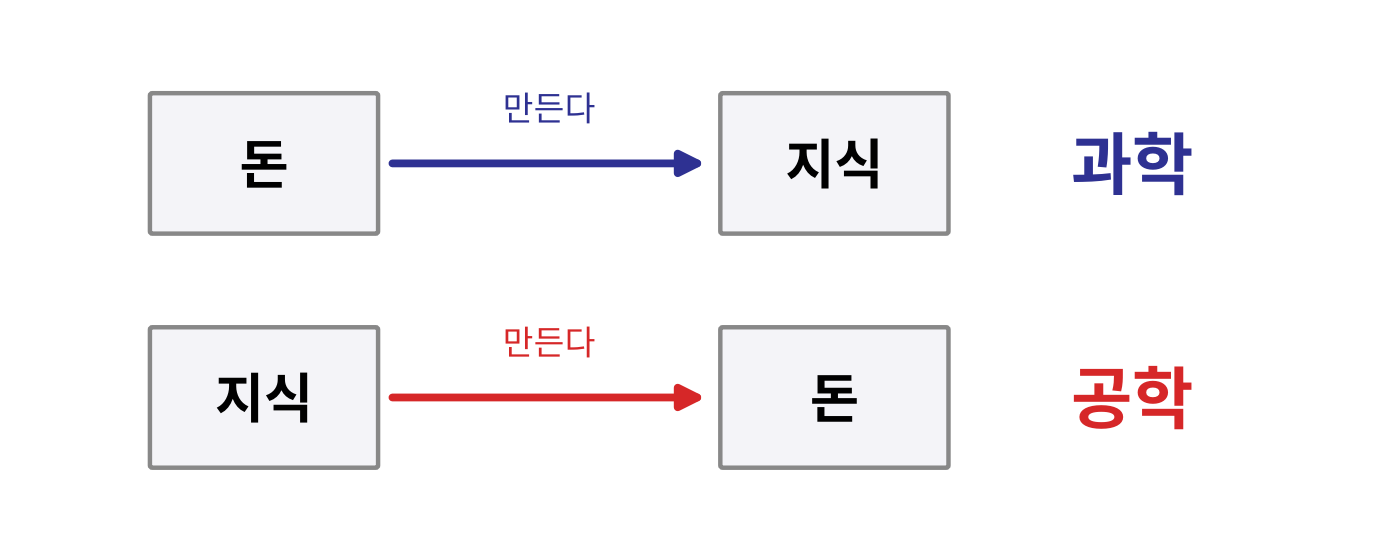
\includegraphics[width=0.66\linewidth]{intro_sci_eng.png}\par\vskip0.4em
{\small 과학은 돈으로 지식을 만들고, 공학은 지식으로 돈을 만든다}
\vfill
\note{조금 가볍게 말하면 이런 우스갯소리도 있습니다. 과학은 돈을 써서 지식을 만드는 일이고, 공학은 지식을 써서 돈을 만드는 일이다. 농담이지만 방향이 반대라는 점은 꽤 정확합니다. 이 두 화살표를 기억하면서 역사를 보겠습니다.}
\end{frame}

% --- 1943
\begin{frame}{1943: 뉴런을 흉내 낸 회로}
\vfill
\centering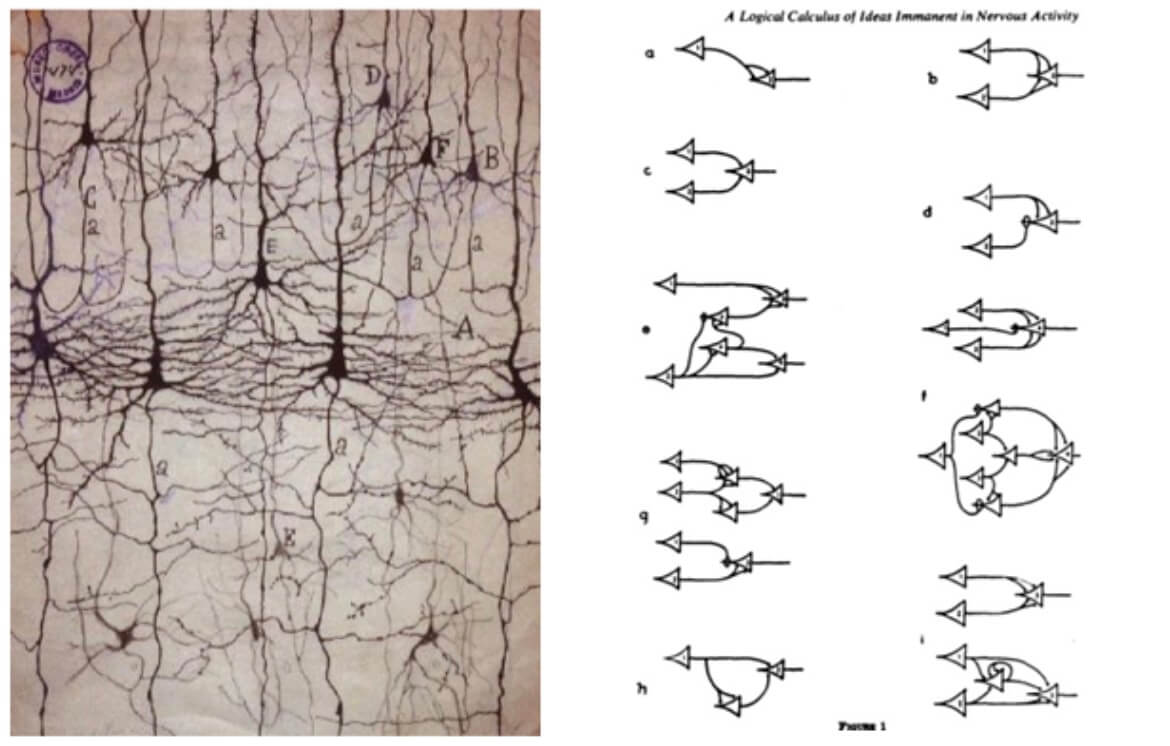
\includegraphics[width=0.64\linewidth]{neuron_history.jpg}\par\vskip0.4em
{\small 왼쪽: 카할의 신경세포 그림 (1890년대) \quad 오른쪽: 매컬러와 피츠의 인공 뉴런 (1943)}
\vfill
\note{인공지능의 아이디어는 생각보다 오래됐습니다. 1943년 매컬러와 피츠는 뇌의 신경세포를 흉내 낸 아주 단순한 회로를 제안했습니다. 입력을 더해서 기준을 넘으면 1, 아니면 0을 내는 회로인데, 이것만으로 AND, OR, NOT 같은 논리를 모두 만들 수 있다는 것을 보였습니다. 오늘 수업에서 배울 신경망의 할아버지뻘입니다. 80년도 넘은 아이디어라는 점을 기억해 두세요.}
\end{frame}

% --- 1958 퍼셉트론과 겨울
\begin{frame}{1958: 퍼셉트론, 그리고 두 번의 겨울}
\vfill
\centering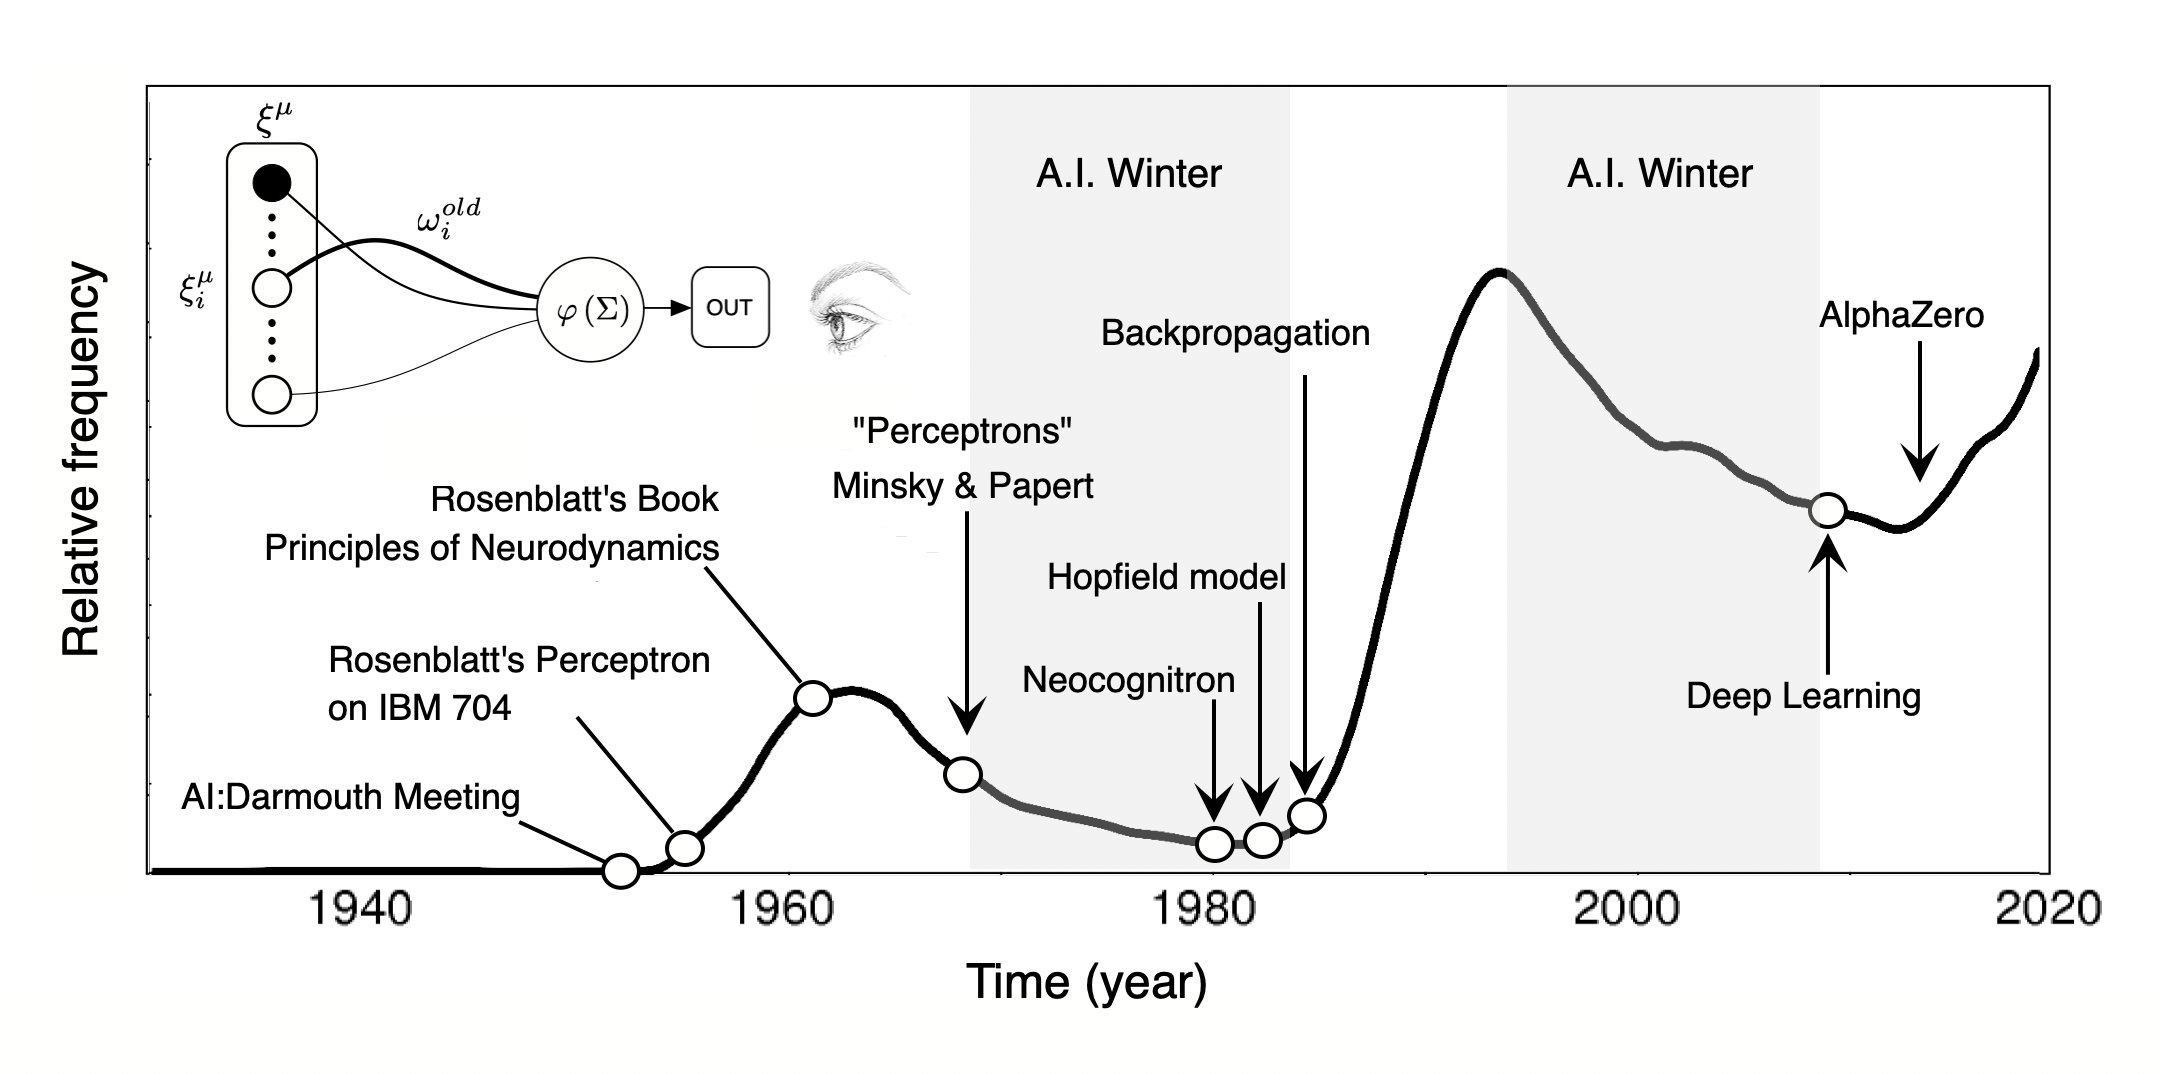
\includegraphics[width=0.66\linewidth]{ai_winters_perceptron.jpg}\par\vskip0.3em
{\small 기대가 커졌다가 실망하고 연구비가 끊기는 ``AI 겨울''이 두 번 왔다}
\vfill
\note{1958년 로젠블랫의 퍼셉트론은 데이터로부터 가중치를 스스로 고치는 첫 학습 기계였고, 신문들은 곧 생각하는 기계가 나온다고 떠들었습니다. 그런데 1969년 민스키와 패퍼트가 퍼셉트론 하나로는 XOR 같은 간단한 문제도 못 푼다는 것을 보이면서 기대가 꺼졌고, 연구비가 끊기는 첫 번째 AI 겨울이 왔습니다. 80년대 후반에 한 번 더 겨울이 옵니다. 기대가 부풀었다가 꺼지는 일이 반복됐다는 점이 중요합니다.}
\end{frame}

% --- 1998 LeNet
\begin{frame}{1998: 손글씨를 읽는 신경망}
\vfill
\centering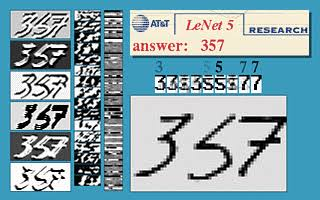
\includegraphics[width=0.62\linewidth]{mnist_demo.jpg}\par\vskip0.4em
{\small 얀 르쿤의 LeNet (합성곱 신경망, CNN) --- 미국에서 수표의 손글씨 숫자를 읽는 데 실제로 쓰였다}
\vfill
\note{겨울 사이에도 연구는 계속됐습니다. 1986년에 역전파가 다시 주목받았고, 1998년 얀 르쿤은 합성곱 신경망 LeNet으로 손글씨 숫자를 읽었습니다. 미국 은행에서 수표를 읽는 데 실제로 쓰였을 정도로 잘 됐습니다. 그런데도 신경망은 2000년대 내내 주류가 아니었습니다. 왜 그랬을까요? 다음 두 장이 답입니다.}
\end{frame}

% --- 2009 ImageNet
\begin{frame}{2009: 데이터 --- ImageNet}
\vfill
\centering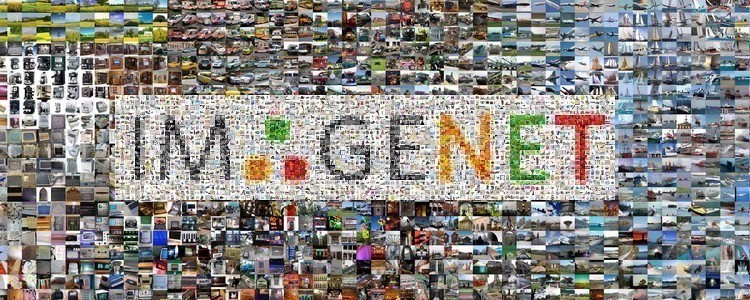
\includegraphics[width=0.66\linewidth]{w01_p2.jpg}\par\vskip0.4em
{\small 페이페이 리 (Stanford): 사진 1,400만 장에 사람이 라벨을 붙였다 (대회용 1,000종 약 128만 장)}
\vfill
\note{첫 번째는 데이터입니다. 페이페이 리는 알고리즘보다 데이터가 부족한 게 문제라고 봤습니다. 그래서 인터넷에서 사진을 모으고, 아마존 메커니컬 터크라는 크라우드소싱 서비스로 전 세계 사람들에게 라벨을 붙이게 해서 1,400만 장짜리 ImageNet을 만들었습니다. 새로운 수학이 아니라, 일을 나눠서 싸게 많이 하는 방법, 즉 공학이었습니다.}
\end{frame}

% --- GPU
\begin{frame}{2007$\sim$2012: 계산 --- 게임용 그래픽카드}
\vfill
\centering
\begin{columns}[c]
\begin{column}{0.40\textwidth}\centering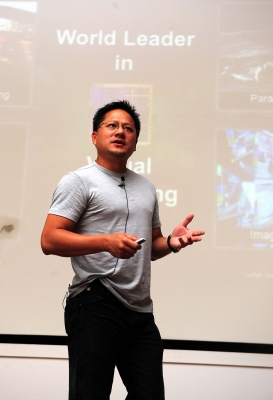
\includegraphics[width=0.66\linewidth]{jensen_huang_snu_2008.jpg}\par\vskip0.2em{\small 젠슨 황, 서울대 강연 (2008)}\end{column}
\begin{column}{0.52\textwidth}\centering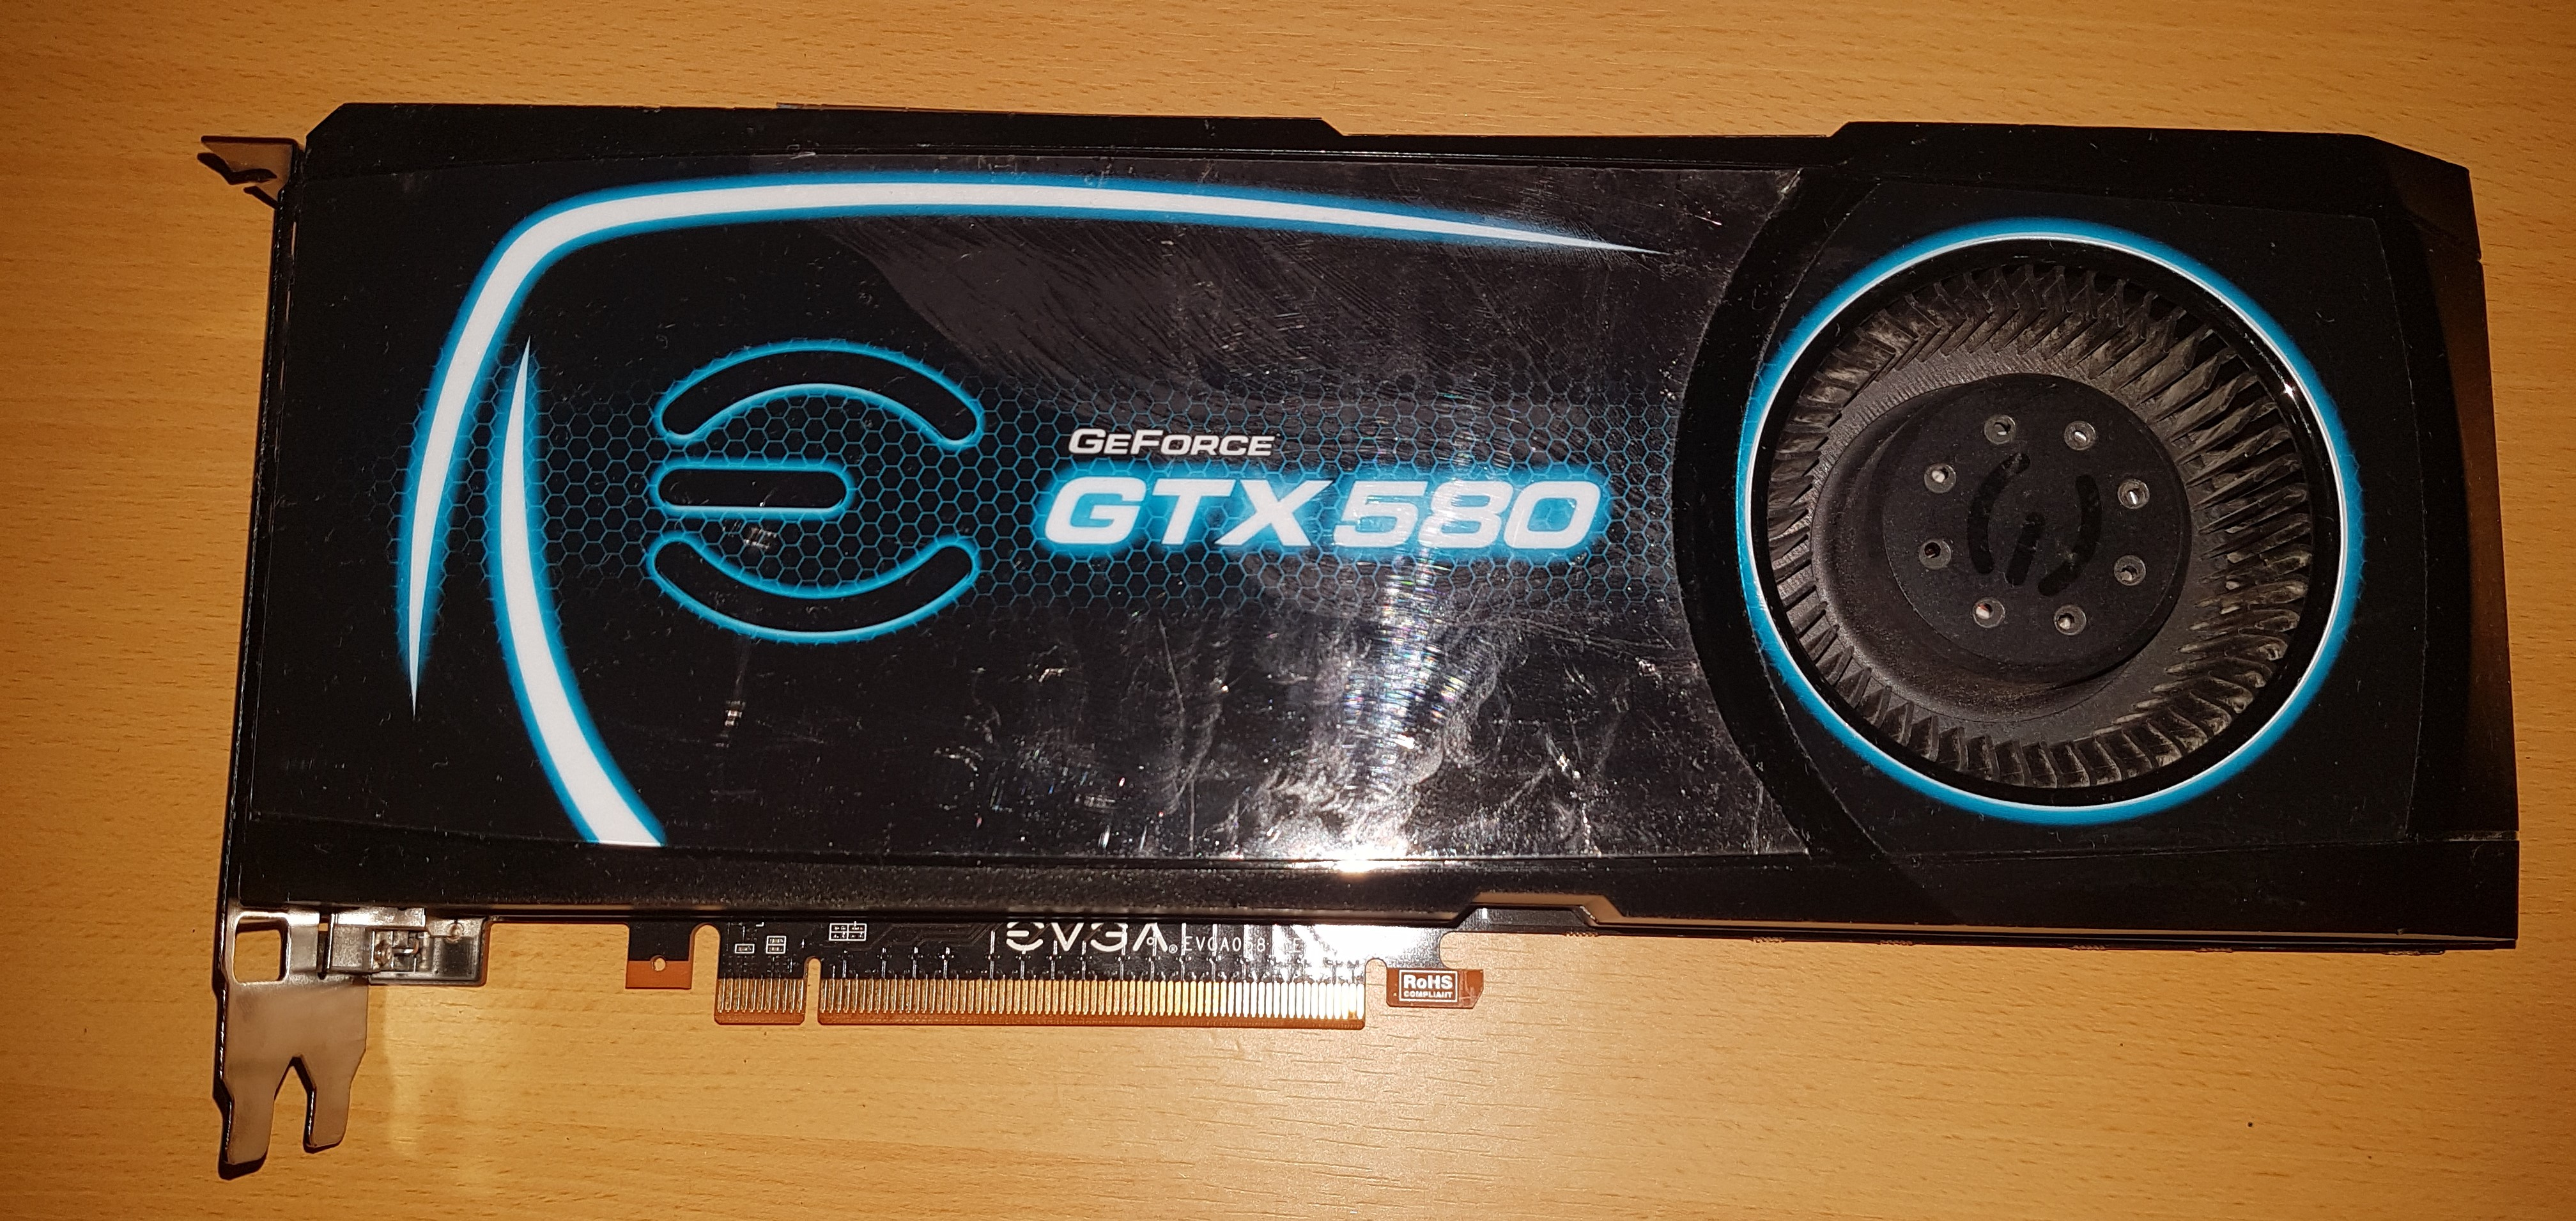
\includegraphics[width=0.82\linewidth]{gtx580.jpg}\par\vskip0.2em{\small GeForce GTX 580 (메모리 3GB)}\end{column}
\end{columns}
\vskip0.6em
{\small 게임 화면을 그리려고 만든 칩이 행렬 곱셈을 수천 개씩 동시에 했다 (2007년 CUDA 공개)}
\vfill
\note{두 번째는 계산입니다. 그래픽카드는 원래 게임 화면을 빠르게 그리려고 만든 칩인데, 그 일이 결국 행렬 곱셈을 엄청나게 많이 동시에 하는 것이었습니다. 신경망 학습도 행렬 곱셈 덩어리입니다. 2007년 엔비디아가 CUDA를 내놓으면서 게임용 칩으로 과학 계산을 할 수 있게 됐습니다. 왼쪽 사진은 2008년 서울대에서 강연하는 젠슨 황입니다. 당시에는 지금처럼 유명한 회사가 아니었습니다.}
\end{frame}

% --- AlexNet
\begin{frame}{2012: AlexNet}
\vfill
\centering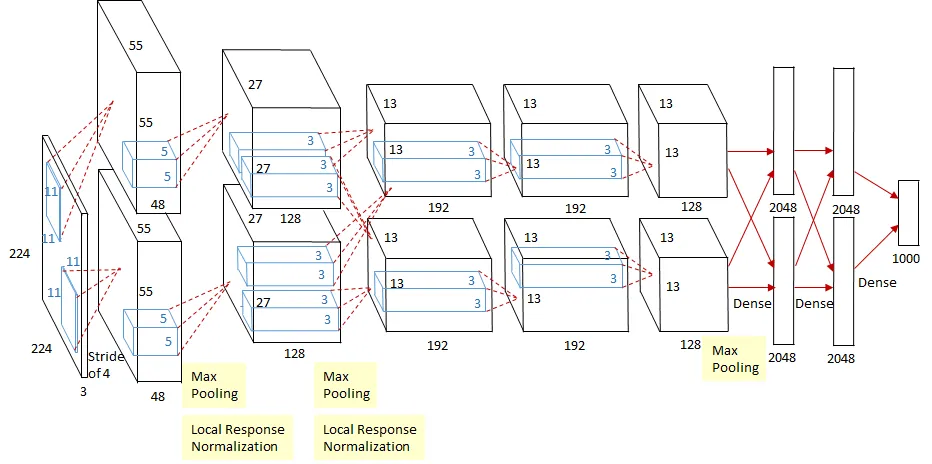
\includegraphics[width=0.78\linewidth]{w01_p3.png}\par\vskip0.4em
{\small 크리제프스키 · 서츠케버 · 힌턴 (토론토대) --- ImageNet 대회 오류율 26\% $\to$ 15\%, GTX 580 두 장으로 약 일주일 학습}
\vfill
\note{2012년, 데이터와 계산이 처음으로 같이 갖춰졌습니다. 토론토대의 크리제프스키, 서츠케버, 힌턴이 만든 AlexNet은 ImageNet 대회에서 2등의 오류율 26퍼센트를 15퍼센트로 끌어내렸습니다. 그림을 보면 신경망이 위아래 두 줄로 나뉘어 있는데, GPU 한 장의 메모리 3기가에 다 안 들어가서 두 장에 반씩 나눠 올린 흔적입니다. 구조 자체는 98년 LeNet과 크게 다르지 않습니다.}
\end{frame}

% --- 연표
\begin{frame}{무엇이 새로웠나}
\markpage{timeline}
\vfill
\centering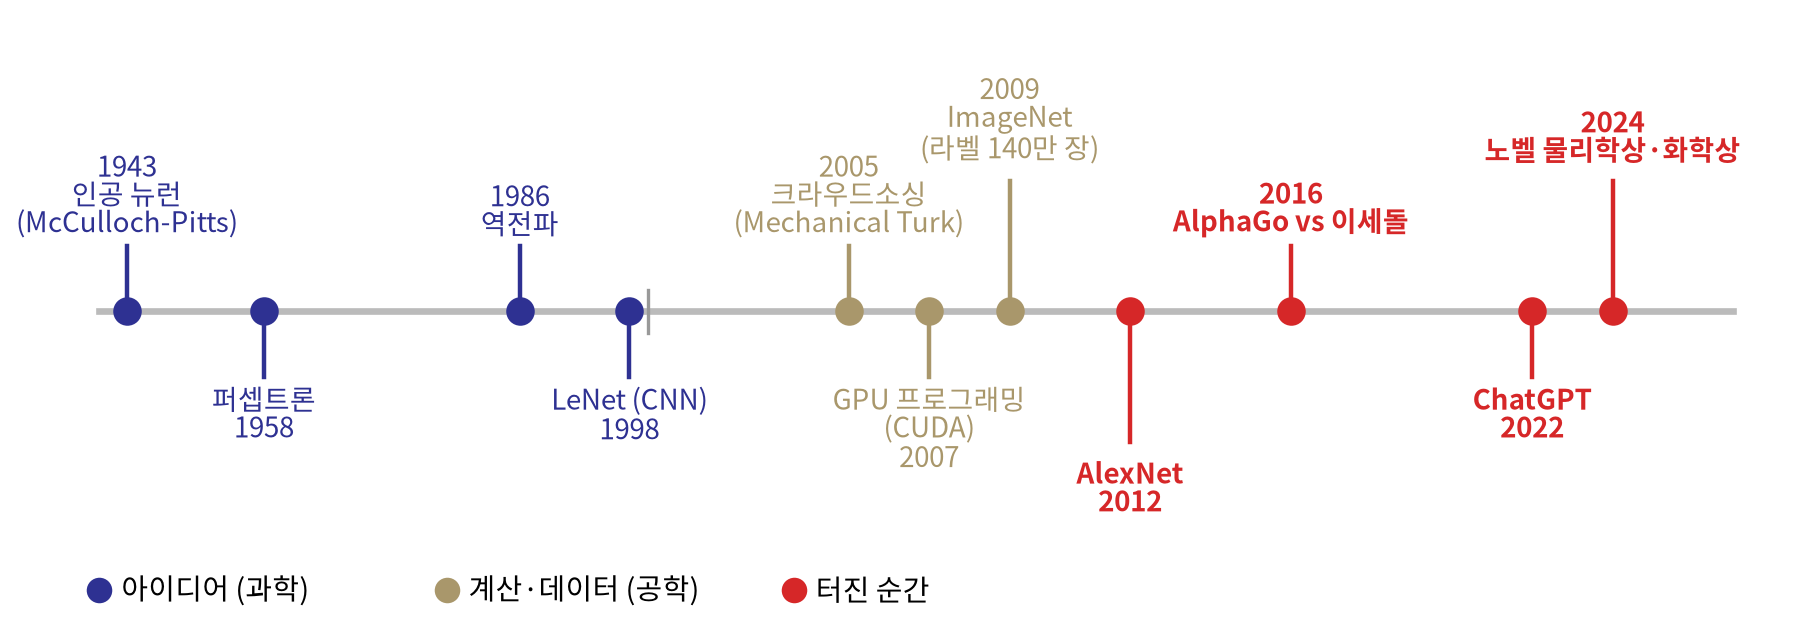
\includegraphics[width=0.96\linewidth]{intro_timeline.png}\par\vskip0.3em
\kq{아이디어는 수십 년 전에 있었다. 터진 것은 계산과 데이터가 갖춰진 뒤였다}
\vfill
\note{연표로 다시 보겠습니다. 파란 점이 아이디어, 금색 점이 계산과 데이터, 빨간 점이 터진 순간입니다. 2000년 이후는 넓게 펼쳐 그렸습니다. 뉴런, 퍼셉트론, 역전파, CNN은 모두 2000년 전에 나왔습니다. 그런데 터진 건 크라우드소싱, GPU, ImageNet이 갖춰진 다음입니다. 그러면 AI는 과학의 산물일까요, 공학의 산물일까요? 적어도 2012년만 보면 공학 쪽 손을 들어 주고 싶어집니다.}
\end{frame}

% --- 쓴 교훈
\begin{frame}{쓴 교훈 (The Bitter Lesson, 2019)}
\vfill
\centering
{\Large ``70년의 AI 연구에서 얻은 가장 큰 교훈은,\\[0.3em]
\kb{계산을 활용하는 일반적인 방법}이 결국 가장 효과적이라는 것이다.''}\par\vskip0.6em
{\footnotesize\itshape\color{gray}``The biggest lesson that can be read from 70 years of AI research is that general methods\\
that leverage computation are ultimately the most effective, and by a large margin.''}\par\vskip0.8em
{\small --- 리치 서튼 (강화학습의 아버지, 2024 튜링상)}\par
{\scriptsize\color{gray} 출처: Rich Sutton, ``The Bitter Lesson'' (2019.\,3.\,13), incompleteideas.net/IncIdeas/BitterLesson.html}\par\vskip1.0em
\kq{사람이 아는 것을 열심히 넣은 방법은, 계산을 더 쓰는 방법에 번번이 졌다}
\vfill
\note{강화학습을 만든 리치 서튼이 2019년에 쓴 짧은 글이 있습니다. 제목이 쓴 교훈입니다. 체스, 바둑, 음성 인식, 이미지 인식에서 연구자들은 사람이 아는 지식을 열심히 넣었는데, 결국은 계산을 많이 쓰는 단순하고 일반적인 방법이 이겼다는 내용입니다. 연구자 입장에서는 쓰라린 이야기라서 쓴 교훈입니다. 이것도 공학 쪽 증거입니다.}
\end{frame}

% --- 불완전해도 돌린다
\begin{frame}{공학은 불완전해도 돌린다}
\vfill
\centering
{\large
\begin{tabular}{l l}
GPU 메모리가 모자란다 & $\to$ 신경망을 두 장에 반씩 나눠 올린다 (AlexNet) \\[0.5em]
왜 잘 되는지 아직 모른다 & $\to$ 일단 돌려 보고, 이해는 나중에 \\[0.5em]
데이터가 부족하다 & $\to$ 사진을 뒤집고 잘라서 늘린다 \\[0.5em]
\end{tabular}}\par\vskip0.8em
\kq{완벽한 이론을 기다리지 않고, 어떻게든 돌아가게 만드는 것}
\vfill
\note{공학의 특징은 완벽해서 굴러가는 게 아니라, 불완전해도 어떻게든 돌아가게 만든다는 점입니다. AlexNet은 메모리가 모자라서 신경망을 두 장에 나눠 올렸고, 딥러닝이 왜 이렇게 잘 되는지는 지금도 완전히 설명하지 못합니다. 그래도 돌려 보고, 되는 것을 찾고, 이해는 나중에 따라옵니다. 이번 학기에 여러분도 이런 경험을 많이 하게 됩니다.}
\end{frame}

% --- 알파고
\begin{frame}{2016, 서울: 알파고 대 이세돌}
\vfill
\centering
\begin{columns}[c]
\begin{column}{0.40\textwidth}\centering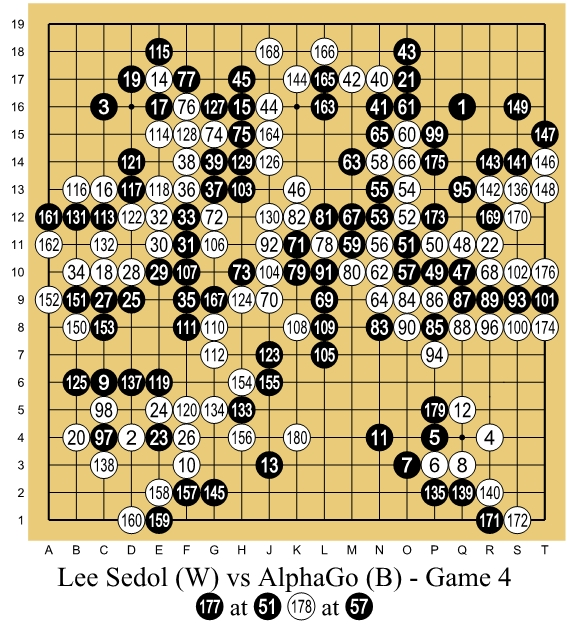
\includegraphics[width=0.92\linewidth]{alphago_game4.jpg}\end{column}
\begin{column}{0.52\textwidth}
\large 딥마인드의 알파고가 4 : 1 로 이겼다\\[0.6em]
\normalsize 그림은 이세돌이 이긴 \kb{4국}의 기보\\[0.3em]
78수: 알파고가 예상하지 못한 한 수\\[1.0em]
\small 데미스 허사비스 --- 게임 개발자 $\to$ 신경과학 박사 $\to$ 딥마인드 창업
\end{column}
\end{columns}
\vfill
\note{2016년 3월, 서울에서 딥마인드의 알파고와 이세돌 9단이 다섯 판을 뒀고 알파고가 4대 1로 이겼습니다. 왼쪽은 이세돌이 이긴 4국입니다. 78수는 알파고가 거의 예상하지 못한 수였습니다. 딥마인드를 세운 데미스 허사비스는 게임 개발자였다가 신경과학으로 박사를 받고 회사를 만든 사람입니다. 한국에서 일어난 일이라 여러분 기억에도 남아 있을 겁니다.}
\end{frame}

% --- 노벨상
\begin{frame}{반전: 2024년 노벨상}
\vfill
\centering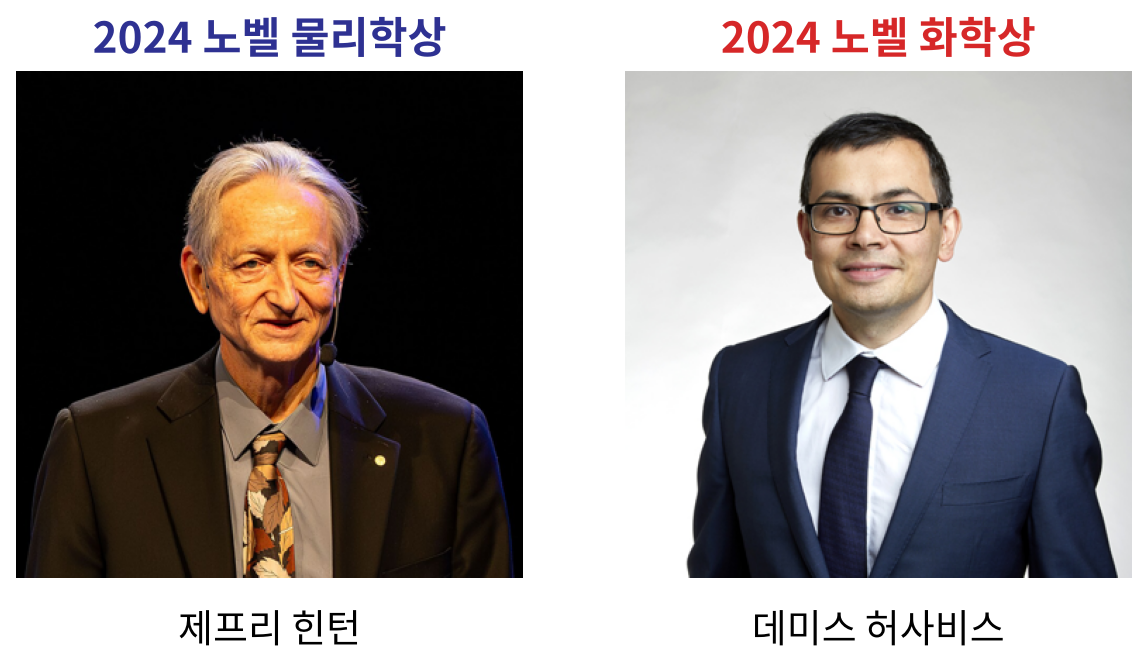
\includegraphics[width=0.52\linewidth]{intro_nobel.png}\par\vskip0.4em
{\small 물리학상: 홉필드 · 힌턴 (신경망) \qquad 화학상: 허사비스 · 점퍼 (알파폴드, 단백질 구조) · 베이커}\par\vskip0.4em
\kq{공학처럼 보이던 AI가 과학의 상을 받았다}
\vfill
\note{그런데 반전이 있습니다. 2024년 노벨 물리학상은 신경망을 만든 홉필드와 힌턴이 받았고, 노벨 화학상의 절반은 단백질 구조를 예측하는 알파폴드를 만든 허사비스와 점퍼가 받았습니다. 공학의 산물처럼 보이던 AI가 과학의 가장 큰 상을 두 개나 받은 겁니다. 첫 장의 파인먼 문장을 떠올려 보세요. 만들어 보는 것이 곧 이해하는 방법일 수도 있습니다. 그러면 다시, AI는 과학일까요, 공학일까요? 정답이 있는 질문은 아닙니다. 학기 내내 생각해 보세요.}
\end{frame}

% --- 토론
\begin{frame}{토론: 과학의 산물인가, 공학의 산물인가}
\markpage{debate}
\vfill
\begin{columns}[T]
\begin{column}{0.47\textwidth}
\centering{\Large\kb{과학의 산물이다}}\par\vskip0.6em
\begin{itemize}
\item 신경망 · 역전파는 수학에서 나왔다
\item 노벨 물리학상 · 화학상
\item 알파폴드가 \textbf{자연}(단백질)을 밝혔다
\item 왜 되는지 밝히는 연구가 계속된다
\end{itemize}
\end{column}
\begin{column}{0.47\textwidth}
\centering{\Large\kq{공학의 산물이다}}\par\vskip0.6em
\begin{itemize}
\item 터진 건 GPU와 데이터 덕분 \pref{timeline}
\item 계산을 더 쓰는 쪽이 늘 이겼다
\item 왜 되는지 몰라도 일단 돌린다
\item 만들 줄 알지만 이해는 아직 \pref{question}
\end{itemize}
\end{column}
\end{columns}
\vskip1.0em
\centering\kq{여러분은 어느 쪽인가? 근거 하나를 들어 말해 보자}
\vfill
\note{여기서 잠깐 토론을 해 보겠습니다. 왼쪽은 과학의 산물이라는 쪽의 근거입니다. 신경망과 역전파, 확률 이론은 수학에서 나왔고, AI가 노벨상을 두 개나 받았고, 알파폴드는 단백질 구조라는 자연을 밝혀냈습니다. 오른쪽은 공학의 산물이라는 쪽입니다. 아이디어는 수십 년 전에 있었고 터진 건 GPU와 데이터가 갖춰진 뒤였고, 계산을 더 쓰는 방법이 늘 이겼고, 왜 되는지 몰라도 일단 돌려서 씁니다. 몇 명에게 어느 쪽인지, 근거 하나를 들어 말해 보게 하세요. 토론이 끝난 뒤에 제 생각을 말하면, 저는 공학 쪽에 더 가깝다고 봅니다. 우리가 AI를 만들 줄은 알지만 아직 이해하지는 못했기 때문입니다. 다만 그렇게 만든 AI가 이제는 과학을 하는 도구가 되고 있습니다. 정답이 있는 질문은 아닙니다.}
\end{frame}

% --- 사람들
\begin{frame}{이번 학기에 자주 만날 사람들}
\vfill
\centering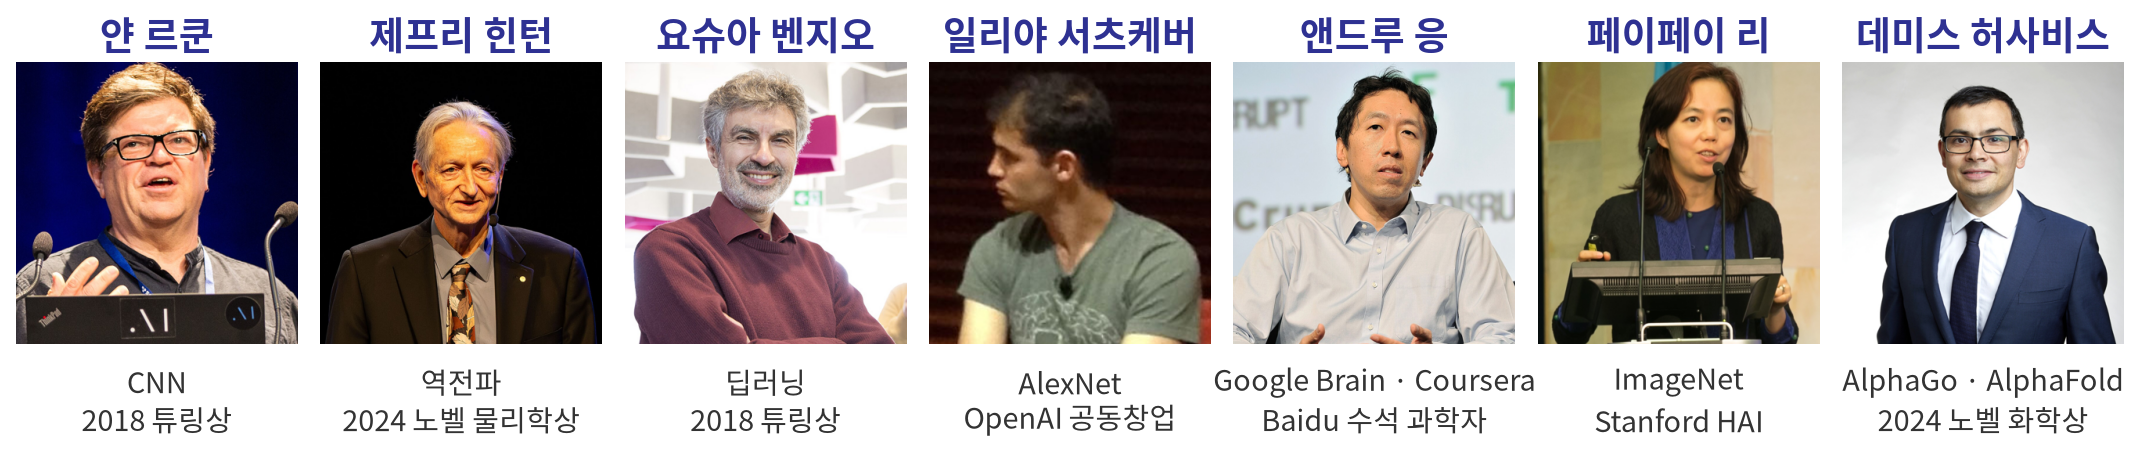
\includegraphics[width=\linewidth]{intro_people.png}
\vfill
\note{이번 학기에 자주 이름이 나올 사람들입니다. CNN의 르쿤, 역전파의 힌턴, 두 사람과 함께 2018년 튜링상을 받은 벤지오가 딥러닝의 세 대부로 불립니다. 서츠케버는 AlexNet을 만들고 OpenAI를 같이 세웠습니다. 앤드루 응은 구글 브레인을 만들고, 코세라로 온라인 강의를 퍼뜨렸고, 2014년부터 3년간 바이두의 수석 과학자로 일했습니다. 페이페이 리는 ImageNet을, 허사비스는 알파고와 알파폴드를 만들었습니다. 각 주제를 배울 때 이 사람들이 다시 나옵니다.}
\end{frame}

% --- 실리콘밸리
\begin{frame}{연구실에서 회사로: 실리콘밸리의 문화}
\vfill
\centering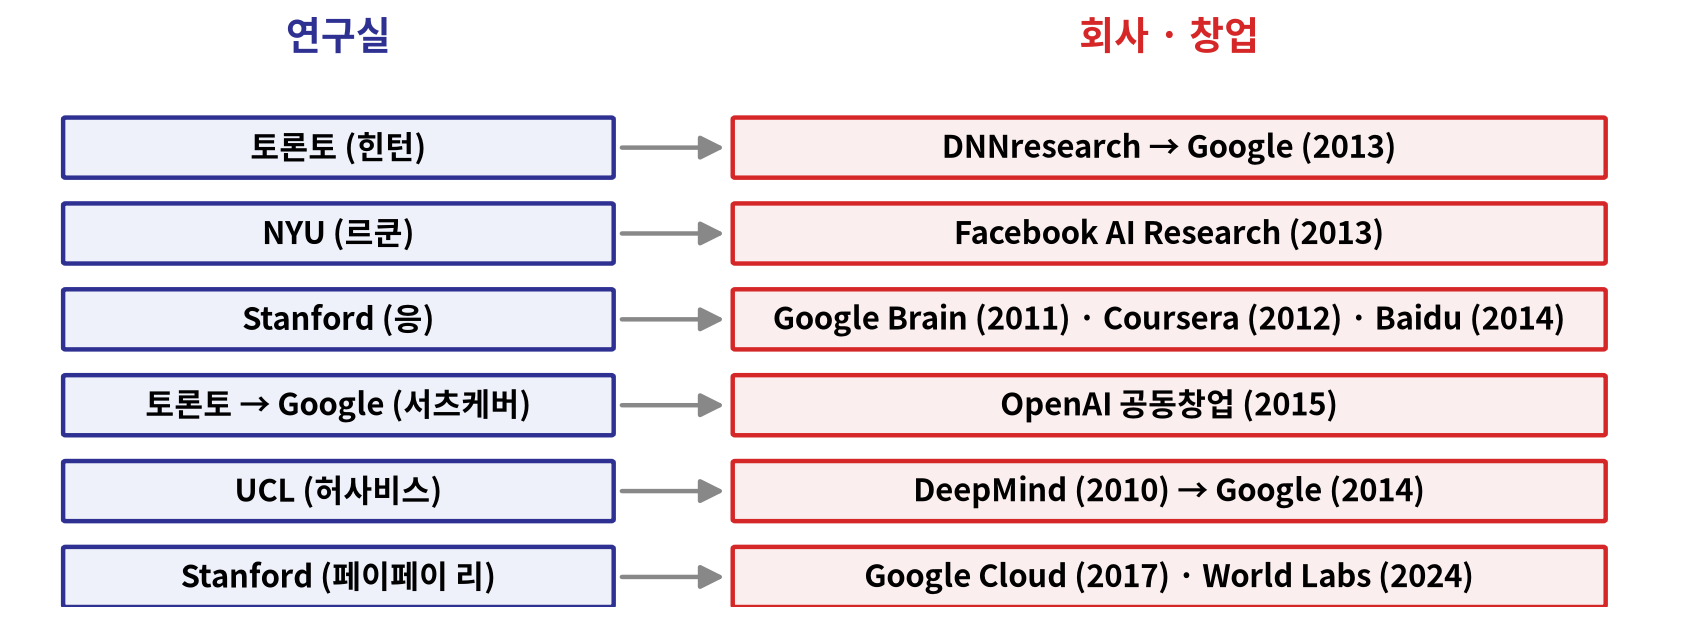
\includegraphics[width=0.72\linewidth]{intro_valley.png}\par\vskip0.3em
{\small 논문은 arXiv에 바로 공개, 코드는 GitHub에 공개 $\to$ 고등학생도 최신 연구를 바로 따라 할 수 있다}
\vfill
\note{이 사람들 대부분이 대학 연구실에서 시작해 회사로 가거나 회사를 세웠습니다. 힌턴의 연구실은 구글에 인수됐고, 르쿤은 페이스북 AI 연구소를, 응은 구글 브레인과 코세라를 만들고 중국 바이두의 수석 과학자로도 일했고, 허사비스는 딥마인드를 만들었습니다. 연구가 곧바로 제품이 되는 이 문화가 실리콘밸리의 특징입니다. 또 하나는 열린 문화입니다. 논문은 심사 전에도 arXiv에 올리고, 코드는 GitHub에 공개합니다. 그래서 여러분도 지금 바로 최신 연구를 따라 할 수 있습니다.}
\end{frame}

% --- 이 수업은
\begin{frame}{그래서 이 수업은}
\vfill
\centering
{\Large 어려운 개념을 \textbf{외우는} 수업이 아니다}\par\vskip1.0em
{\Large \kq{AI를 도구로 써서, 자기 데이터로 실험하고,}\\[0.4em]
\kq{논문을 써서 동료 평가를 받는 수업}}\par\vskip1.0em
{\small 기초 개념은 배운다. 하지만 목표는 개념이 아니라 \textbf{직접 해 보는 경험}}
\vfill
\note{그래서 이 수업은 어려운 개념을 외우는 수업이 아닙니다. 기초 개념은 배우고 이야기하겠지만, 목표는 여러분이 직접 해 보는 겁니다. AI를 도구로 써서 자기가 연구하고 싶은 데이터를 찾고, 실험하고, 논문을 써서 동료 평가를 받는 수업입니다.}
\end{frame}

% --- 학기 흐름
\begin{frame}{한 학기 동안 할 일}
\vfill
\centering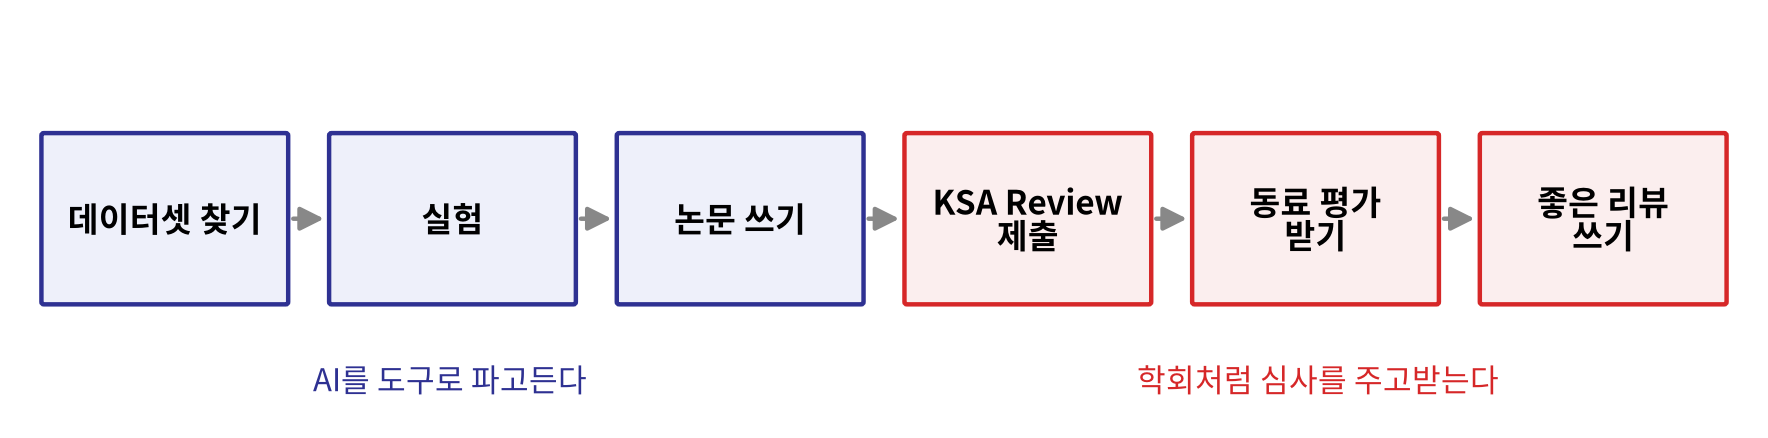
\includegraphics[width=0.96\linewidth]{intro_course_flow.png}\par\vskip0.4em
{\small KSA Review: 학회처럼 논문을 제출하고, 서로 심사하고, 반박하는 우리 수업의 심사 사이트}\par\vskip0.4em
\kb{좋은 리뷰를 쓰는 것도 이 수업에서 배우는 것이다}
\vfill
\note{한 학기 흐름입니다. 각자 AI를 활용해 연구하고 싶은 데이터셋을 찾고, 실험하고, 논문 형태로 씁니다. 그리고 KSA Review라는 우리 수업의 심사 사이트에 실제 학회처럼 제출해서 동료 평가를 받습니다. 중요한 건 오른쪽 끝입니다. 평가를 받는 것만큼 양질의 평가를 하는 것도 이 수업에서 얻어 가야 할 경험입니다.}
\end{frame}

% --- 리뷰어는 무엇을 보나
\begin{frame}{리뷰어는 무엇을 보나}
\vfill
\centering
{\large
\begin{tabular}{r l}
\kb{1} & 주장이 실험 결과와 맞는가? \\[0.5em]
\kb{2} & 비교 대상(베이스라인)이 있는가? \\[0.5em]
\kb{3} & 시험 데이터가 학습에 새지 않았는가? \\[0.5em]
\kb{4} & 다른 사람이 다시 해 볼 수 있는가? \\[0.5em]
\kb{5} & 한계를 솔직하게 적었는가? \\
\end{tabular}}\par\vskip0.8em
\kq{``좋아요''가 아니라, 저자가 반박할 수 있는 질문을 쓴다}
\vfill
\note{ML 논문의 리뷰어들이 실제로 보는 것은 대체로 이 다섯 가지입니다. 주장이 결과와 맞는지, 비교할 기준이 있는지, 시험 데이터가 학습에 새지 않았는지, 다른 사람이 다시 해 볼 수 있는지, 한계를 솔직하게 적었는지. 좋은 리뷰는 "잘 썼어요"가 아니라 저자가 답할 수 있는 구체적인 질문입니다. 학기 중간과 끝에 이 기준으로 서로 심사합니다.}
\end{frame}

% --- 현실 문제 1
\begin{frame}{현실 문제 1: 정확도 90\%의 함정}
\markpage{cancer}
\vfill
\begin{columns}[c]
\begin{column}{0.44\textwidth}\centering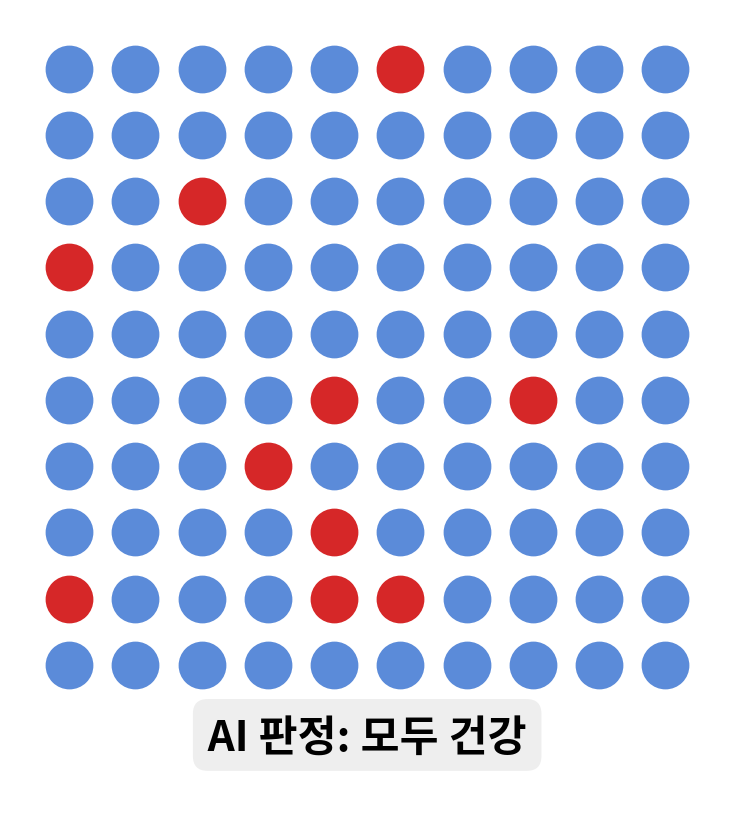
\includegraphics[width=0.9\linewidth]{intro_acc_trap.png}\end{column}
\begin{column}{0.52\textwidth}
{\large 100명 중 \textcolor{ksared}{\textbf{환자 10명}}}\\[0.8em]
AI가 \textbf{모두 건강}이라고 찍으면\\[0.4em]
{\LARGE\kb{정확도 90\%}}\\[0.6em]
{\large 그런데 환자는 \kq{한 명도 못 찾았다}}\\[1.0em]
{\small 쏠린(불균형) 데이터에서는 정확도가 속인다}
\end{column}
\end{columns}
\vfill
\note{이번 학기는 개념보다 실험하면서 실제로 부딪히는 문제들을 다룹니다. 첫 번째 예입니다. 100명 중 환자가 10명입니다. 어떤 AI가 누구에게나 건강하다고 말합니다. 건강한 90명을 다 맞혔으니 정확도 90퍼센트입니다. 그런데 환자는 한 명도 못 찾았습니다. 이렇게 라벨이 한쪽으로 쏠린 데이터를 불균형 데이터라고 하는데, 이럴 때 정확도 하나만 보면 쉽게 속습니다.}
\end{frame}

% --- 현실 문제 1 (이어서)
\begin{frame}{놓치지 않았나, 헛짚지 않았나}
\vfill
\begin{columns}[c]
\begin{column}{0.52\textwidth}\centering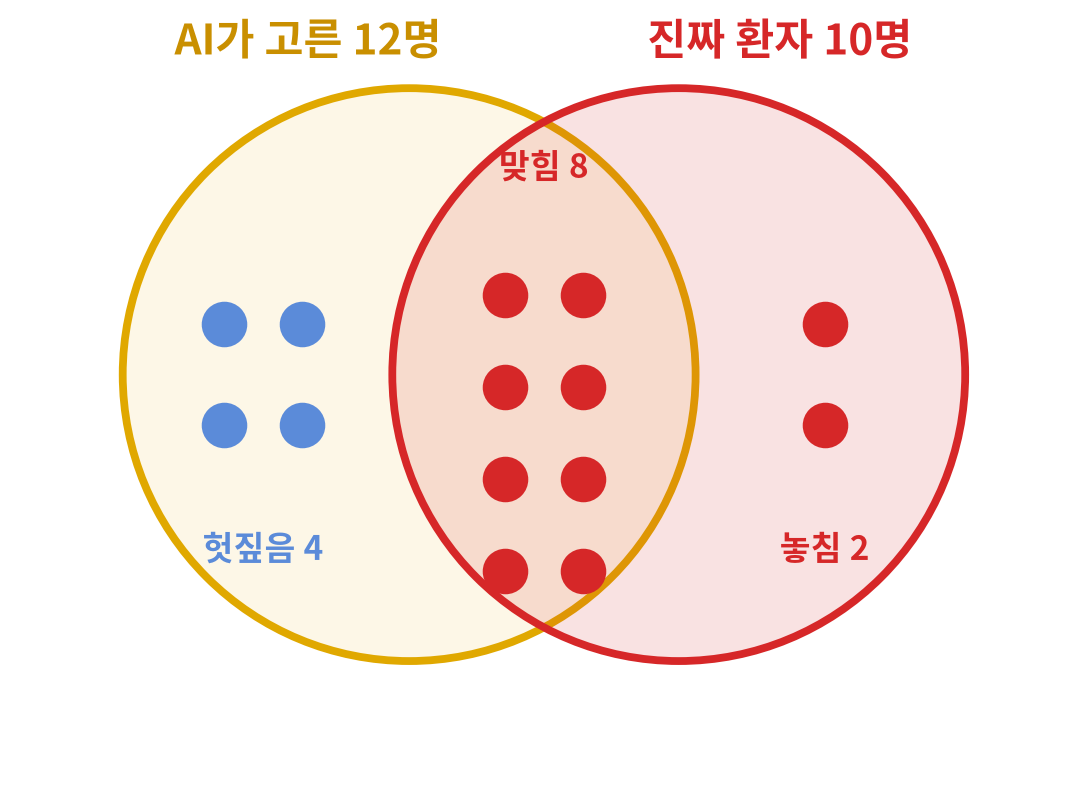
\includegraphics[width=\linewidth]{intro_recall.png}\end{column}
\begin{column}{0.44\textwidth}
{\large 진짜 AI가 12명을 환자로 골랐다}\\[1.0em]
\kq{재현율} (Recall) $= 8 \div 10 = $ \textbf{80\%}\\[0.2em]
{\small 진짜 환자 중 몇 명을 찾았나? (놓침)}\\[0.9em]
\kb{정밀도} (Precision) $= 8 \div 12 \approx$ \textbf{67\%}\\[0.2em]
{\small 환자라고 한 사람 중 진짜는? (헛짚음)}\\[0.9em]
{\small 무엇이 더 중요한지는 문제마다 다르다 (2주차)}
\end{column}
\end{columns}
\vfill
\note{그래서 다른 잣대가 필요합니다. 진짜 AI가 100명 중 12명을 환자로 골랐다고 합시다. 그중 8명은 진짜 환자이고, 4명은 건강한데 잘못 골랐고, 환자 2명은 놓쳤습니다. 재현율은 진짜 환자 10명 중 찾아낸 8명, 80퍼센트입니다. 놓치지 않았느냐는 질문입니다. 정밀도는 환자라고 고른 12명 중 진짜 8명, 67퍼센트입니다. 헛짚지 않았느냐는 질문입니다. 암 검사라면 놓치는 게 더 무섭고, 스팸 필터라면 정상 메일을 헛짚는 게 더 곤란합니다. 2주차에 자세히 다룹니다.}
\end{frame}

% --- 현실 문제 2
\begin{frame}{현실 문제 2: 데이터가 모자라면}
\vfill
\centering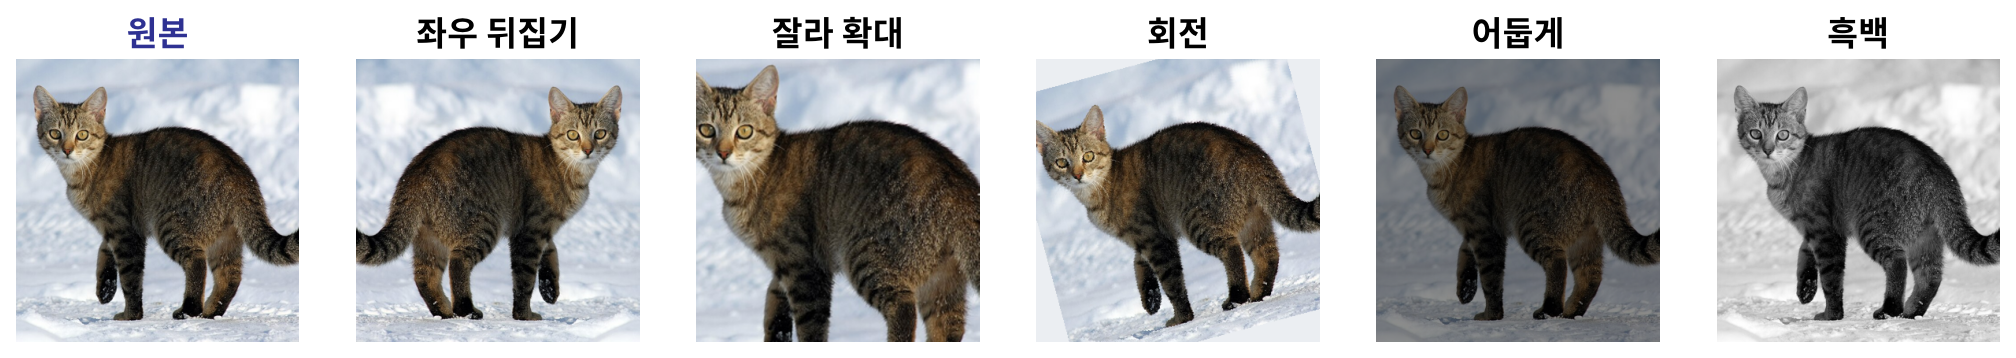
\includegraphics[width=0.96\linewidth]{intro_augment.png}\par\vskip0.4em
{\small 사진 한 장을 뒤집고, 자르고, 돌리고, 어둡게 해서 ``다른'' 학습 데이터로 쓴다 --- 데이터 증강}\par\vskip0.4em
\kb{고양이는 뒤집어도 고양이다: 정답이 바뀌지 않는 변형만 쓴다}
\vfill
\note{두 번째는 데이터 부족입니다. 여러분이 직접 모을 수 있는 데이터는 ImageNet처럼 크지 않습니다. 그럴 때 쓰는 방법이 데이터 증강입니다. 사진 한 장을 뒤집고, 자르고, 돌리고, 밝기를 바꿔서 여러 장처럼 씁니다. 단, 정답이 바뀌지 않는 변형만 써야 합니다. 고양이는 뒤집어도 고양이지만, 숫자 6을 뒤집으면 9가 됩니다.}
\end{frame}

% --- 현실 문제 3
\begin{frame}{현실 문제 3: 딥러닝 없이도}
\vfill
\centering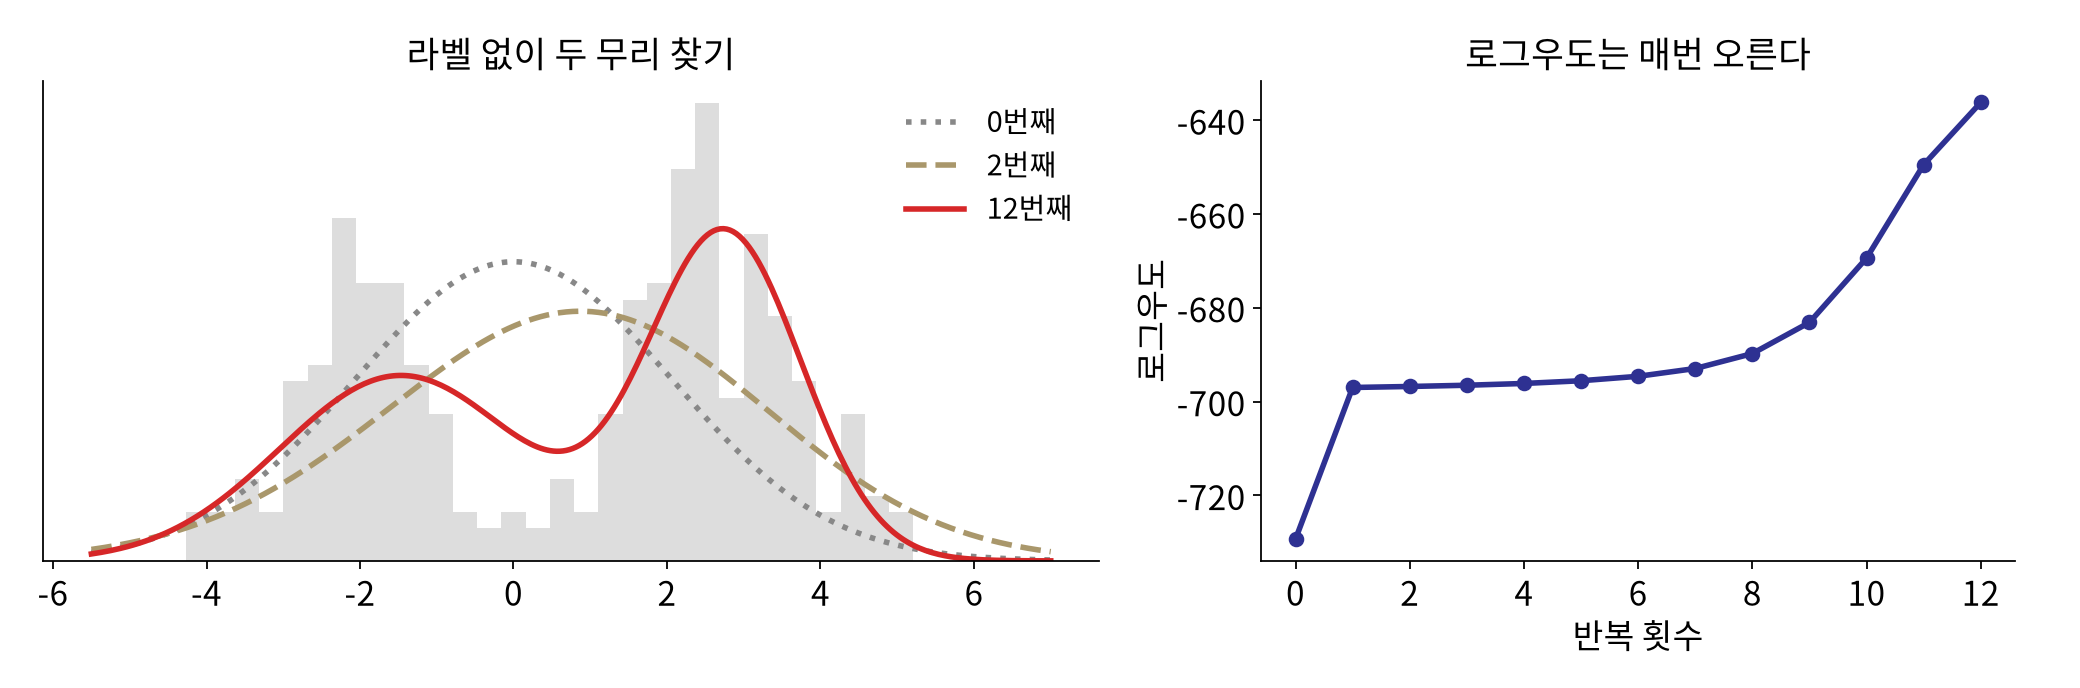
\includegraphics[width=0.86\linewidth]{intro_em.png}\par\vskip0.3em
{\small 라벨 없는 데이터에서 두 무리를 찾는 EM 알고리즘 --- 반복할 때마다 로그우도가 오른다 (4주차)}
\vfill
\note{세 번째는 딥러닝이 없던 시절의 방법들입니다. 데이터가 적거나 라벨이 없을 때는 오히려 이런 방법이 낫습니다. 그림은 라벨 없이 점들을 두 무리로 나누는 EM 알고리즘입니다. 처음에는 엉뚱한 곳에 두 봉우리를 놓지만, 반복할수록 데이터에 맞춰지고, 오른쪽처럼 로그우도라는 점수가 한 번도 줄지 않고 오릅니다. 4주차에 직접 손으로 해 봅니다.}
\end{frame}

% --- 현실 문제 3 (이어서): 표 데이터
\begin{frame}{표 데이터에서는 아직도 트리가 이긴다}
\vfill
\centering
{\small 예: 카드 사기거래 탐지 --- 거래 한 건 = 표의 한 줄}\par\vskip0.4em
{\footnotesize
\begin{tabular}{r r l l c}
\hline
금액(원) & 시각 & 가맹점 & 기기 & 사기? \\
\hline
12{,}000 & 13:05 & 편의점 & 늘 쓰던 폰 & 아니오 \\
2{,}450{,}000 & 03:41 & 해외 온라인 & 처음 보는 PC & \textcolor{ksared}{\textbf{예}} \\
58{,}000 & 19:20 & 식당 & 늘 쓰던 폰 & 아니오 \\
\hline
\end{tabular}}\par\vskip0.8em
{\large 이런 \kb{표(tabular) 데이터}에서는 딥러닝보다\\[0.2em]
\kq{GBDT} (XGBoost, LightGBM, CatBoost) 가 아직도 잘 나온다}\par\vskip0.6em
{\small Kaggle IEEE-CIS 사기거래 탐지 대회(2019) 1등도 GBDT 세 가지를 섞은 모델 (7주차)}\par\vskip0.6em
{\tiny 출처: Grinsztajn, Oyallon \& Varoquaux, ``Why do tree-based models still outperform deep learning on typical tabular data?'' (NeurIPS 2022);\\
Shwartz-Ziv \& Armon, ``Tabular data: Deep learning is not all you need'' (Information Fusion, 2022);
Kaggle ``IEEE-CIS Fraud Detection'' (2019) 1등 풀이}
\vfill
\note{딥러닝이 아닌 방법이 이기는 곳이 또 있습니다. 표 데이터입니다. 카드 사기거래 탐지를 생각해 봅시다. 거래 한 건이 표의 한 줄이고, 금액, 시각, 가맹점, 기기 같은 칸이 있습니다. 회사와 병원, 은행에서 다루는 데이터는 대부분 이런 표입니다. 그런데 이런 데이터에서는 지금도 딥러닝보다 GBDT, 즉 결정 트리를 여러 개 이어 붙인 XGBoost, LightGBM, CatBoost 같은 모델이 더 잘 나오는 경우가 많습니다. 2022년 NeurIPS 논문은 45개 표 데이터셋에서 트리 모델이 딥러닝보다 낫다는 것을 보였고, 2019년 캐글 사기거래 탐지 대회의 1등 팀도 이 세 가지 GBDT를 섞어 썼습니다. 최근에는 TabPFN처럼 표 데이터용 신경망이 따라잡는 연구도 나오고 있으니, 무엇이 더 나은지는 여러분이 실험으로 확인해 보세요. 트리와 GBDT는 7주차에 다룹니다.}
\end{frame}

% --- 탑다운
\begin{frame}{AI를 쓰는 법: 바텀업 말고 탑다운}
\vfill
\centering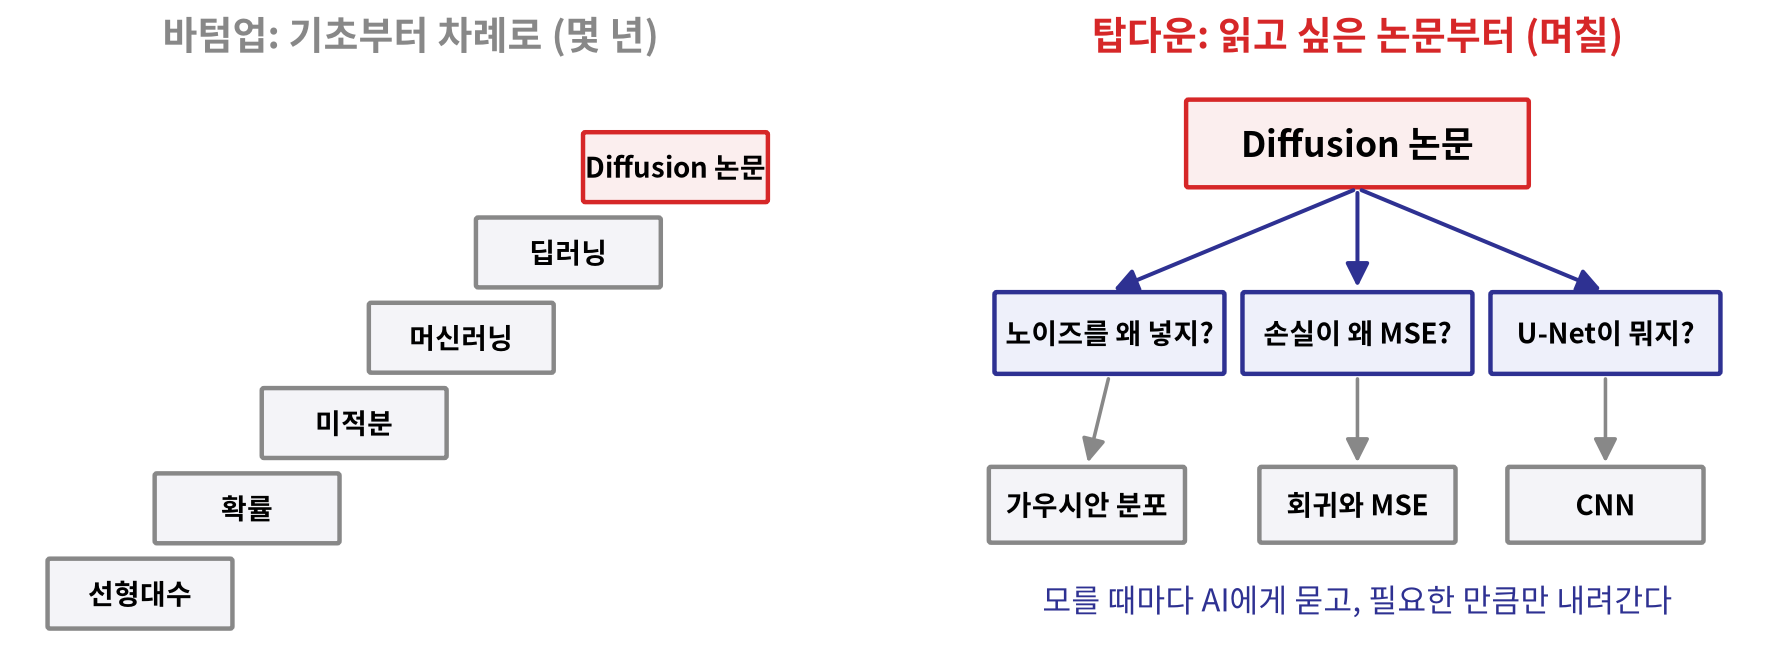
\includegraphics[width=0.92\linewidth]{intro_topdown.png}\par\vskip0.2em
\kq{읽고 싶은 논문을 먼저 정하고, 모르는 것이 나올 때마다 AI에게 묻는다}
\vfill
\note{마지막으로 AI를 어떻게 쓸지입니다. 왼쪽은 우리가 보통 공부하는 방식, 바텀업입니다. 선형대수, 확률, 미적분을 다 배우고 나서야 논문을 읽습니다. 몇 년이 걸립니다. 오른쪽은 탑다운입니다. 읽고 싶은 논문, 예를 들어 그림을 만드는 Diffusion 논문을 먼저 정하고, 모르는 게 나올 때마다 AI에게 묻고, 필요한 만큼만 내려갑니다. OpenAI의 한 연구원은 인터뷰에서 이렇게 해서 대학 몇 년치 공부를 며칠 만에 따라잡았다고 말했습니다. AI는 숙제를 대신하는 도구가 아니라 이렇게 파고드는 도구로 쓰세요.}
\end{frame}

% --- 로드맵
\begin{frame}{이번 학기 17주}
\vfill
\centering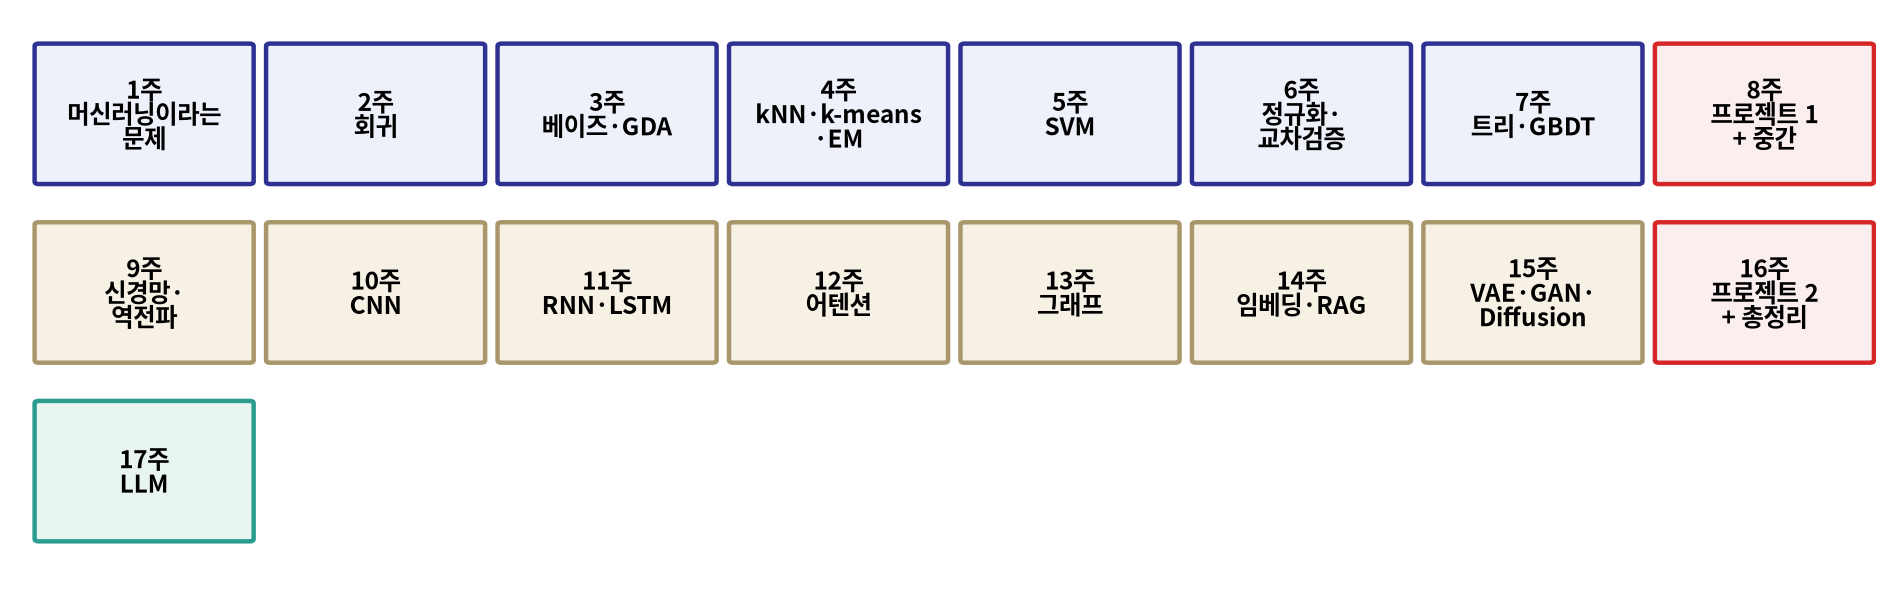
\includegraphics[width=0.96\linewidth]{intro_roadmap.png}\par\vskip0.3em
{\small 파랑: 고전 ML \quad 금색: 신경망과 생성모델 \quad 빨강: 프로젝트 (논문 · 동료 평가) \quad 초록: LLM}
\vfill
\note{이번 학기 17주입니다. 전반부는 회귀, 베이즈, SVM, 트리 같은 고전 머신러닝이고, 8주차에 첫 프로젝트가 있습니다. 후반부는 신경망, CNN, RNN, 어텐션, 생성모델이고, 16주차에 두 번째 프로젝트가 있습니다. 마지막 17주차에는 LLM을 다룹니다. 프로젝트 두 번이 앞에서 말한 논문과 동료 평가입니다.}
\end{frame}

% --- 첫 과제
\begin{frame}{첫 과제: 탑다운으로 시작하기}
\vfill
\centering
{\large
\begin{tabular}{r l}
\kb{1} & 읽고 싶은 ML 논문 \textbf{1편}을 고른다 \\[0.5em]
\kb{2} & 그 논문을 AI와 함께 읽으며, 모르는 개념 \textbf{3개}를 적는다 \\[0.5em]
\kb{3} & 내가 실험해 보고 싶은 공개 데이터셋 \textbf{1개}를 찾는다 \\
\end{tabular}}\par\vskip0.8em
{\small 데이터셋 찾는 곳: Kaggle, UCI Machine Learning Repository, Hugging Face Datasets}
\vfill
\note{첫 과제입니다. 읽고 싶은 머신러닝 논문 한 편을 고르세요. 어렵거나 유명하지 않아도 됩니다. 그 논문을 AI와 함께 읽으면서 모르는 개념 세 개를 적어 오세요. 그리고 학기 프로젝트에서 실험해 보고 싶은 공개 데이터셋을 하나 찾아 오세요. 캐글, UCI, 허깅페이스에서 찾을 수 있습니다. 이 세 가지가 학기 내내 쓸 출발점입니다.}
\end{frame}

% --- 정리
\begin{frame}{정리}
\vfill
\centering\large\begin{tabular}{l}
아이디어는 오래됐고, 계산과 데이터가 갖춰지자 터졌다\\[0.5em]
공학은 불완전해도 돌린다 --- 그런데 노벨상도 받았다\\[0.5em]
이 수업: 데이터셋 $\to$ 실험 $\to$ 논문 $\to$ 동료 평가 $\to$ 좋은 리뷰\\[0.5em]
AI는 탑다운으로 파고드는 도구\\
\end{tabular}\par\vskip1.0em
\kq{AI는 과학의 산물일까, 공학의 산물일까?}
\vfill
\note{정리합니다. AI의 아이디어는 오래됐고, 계산과 데이터가 갖춰지자 터졌습니다. 공학은 불완전해도 돌리는 것인데, 그렇게 만든 AI가 노벨상까지 받았습니다. 이 수업에서는 데이터셋을 찾고, 실험하고, 논문을 쓰고, 동료 평가를 받고, 좋은 리뷰를 씁니다. AI는 탑다운으로 파고드는 도구로 쓰세요. 처음 질문으로 돌아가서, AI는 과학의 산물일까요, 공학의 산물일까요? 정답은 없습니다. 학기 내내 각자 생각해 보세요.}
\end{frame}

% --- 이미지 출처
\begin{frame}{이미지 출처}
\begin{center}\begin{varwidth}{0.92\textwidth}\usebeamercolor[fg]{normal text}
  \scriptsize
  \begin{itemize}
    \item 인물 사진 (Wikimedia Commons): 르쿤 --- Jérémy Barande (CC BY-SA 2.0); 힌턴 --- Arthur Petron (CC BY-SA 4.0);
      벤지오 --- Maryse Boyce (CC BY 4.0); 서츠케버 --- Steve Jurvetson, ``Naveen Rao and Ilya Sutskever Stanford 2014'' (CC BY 2.0);
      응 --- TechCrunch (CC BY 2.0); 페이페이 리 --- ITU Pictures (CC BY 2.0); 허사비스 --- Duncan.Hull (CC BY-SA 4.0)
    \item 알파고 대 이세돌 4국 기보 --- Wesalius, Wikimedia Commons (CC BY-SA 4.0)
    \item 고양이 사진 (데이터 증강) --- Von.grzanka, ``Felis catus-cat on snow'', Wikimedia Commons (CC BY-SA 3.0)
    \item AI 겨울 연표 --- AI voor Iedereen (KU Leuven), aivooriedereen.cs.kuleuven.be
    \item AlexNet 구조 --- Krizhevsky, Sutskever \& Hinton, ``ImageNet Classification with Deep Convolutional Neural Networks'' (NeurIPS 2012), Figure 2
    \item ImageNet --- Deng et al., ``ImageNet: A Large-Scale Hierarchical Image Database'' (CVPR 2009)
    \item 쓴 교훈 인용 --- Rich Sutton, ``The Bitter Lesson'' (2019), incompleteideas.net
    \item 인용 --- 파인먼: Caltech Archives, 1988년 칠판 사진
    % 출처 확인 필요 (기존 slides/kor/ml1/week01 자료 재사용): neuron_history.jpg, mnist_demo.jpg, jensen_huang_snu_2008.jpg, gtx580.jpg, w01_p2.jpg
  \end{itemize}
\end{varwidth}\end{center}
\end{frame}
\end{document}
